\begin{frame}
\frametitle{Research life cycle}
\note[item]<2>{Artifacts can be omitted. Useful artifacts will be shown and explained}
\note[item]<2>{Artifacts - magnifying glass to see target product}
\note[item]<2>{Requirements artifact. Give example: too wide, to detailed, good}
\begin{figure}
    \resizebox{10.0cm}{!}{
        \includegraphics{images/rlc.png}
        %\input{images/rlc_opt}
    }
\end{figure}
\begin{center}
    \resizebox{10cm}{!}{
    \begin{tikzpicture}
        \node (tbl) {
            \begin{tabularx}{1.7\textwidth}{cXlll}
                \arrayrulecolor{cyan}
                \textbf{\#} & \textbf{Input}& \textbf{Output} & \textbf{Artifacts} & \\
                1 & Idea & Scope, general requirements & Proposal \\
                2 & Scope, proposal & Requirements, design, calendar plan & SRS, SDP, STP, Design Document\footnotemark \\
                3 & Requirements, design & Product & Sources, binaries, documentation, UTR \\
                4 & Sources and binaries & Bug reports, bug fixed source code & STR \\
                5 & Product & Completion report, completion party
            \end{tabularx}
        };
        \begin{pgfonlayer}{background}
            \draw[rounded corners,top color=blue!20,bottom color=blue!40,draw=white] ($(tbl.north west)+(0.14,0)$)  rectangle ($(tbl.north east)-(0.13,0.9)$);
            %\draw[rounded corners,top color=white,bottom color=blue!40,middle color=white,draw=blue!20] ($(tbl.south west) +(0.13,0.2)$) rectangle ($(tbl.south east)-(0.12,0)$);
            \draw[top color=blue!1,bottom color=blue!20,draw=white] ($(tbl.north east)-(0.13,0.6)$) rectangle ($(tbl.south west)+(0.13,0.2)$);
        \end{pgfonlayer}
    \end{tikzpicture}}
\end{center}
\footnotetext[1]{\small Design document depends on chosen development process and could be SDD, HLD/DLD etc}
\end{frame}

\begin{frame}
\frametitle{Product life cycle}

\end{frame}

\begin{frame}
\frametitle{RLC-PLC relation}

\end{frame}
